\chapter{Pruebas}
\markboth{ \thechapter \quad Pruebas}{}

En este capítulo se practicará con diferentes funcionalidades de látex que pueden resultar útiles a la hora de redactar la memoria de un TFG.

\section{Codigos en latex}

Esta primera sección probará a ilustrar en el documento diversos lenguajes de programación con sus correspondientes códigos de ejemplo.

Comenzando por matlab, se muestra un breve programa de prueba.

\begin{lstlisting}[style=Matlab-editor,frame= single, numbers=left,caption={Filtro LMS en MATLAB},captionpos=b]
mu = 0.01;
N = length(x);
y = zeros(N,1);
e = zeros(N,1);
w = zeros(M,1);
% Pepe
for n = M:N
    x_vec = x(n:-1:n-M+1);
    y(n) = w' * x_vec;
    e(n) = d(n) - y(n);
    w = w + mu * x_vec * e(n);
end
\end{lstlisting}

A continuación, se muestra otro ejemplo representando un código de python, pero en esta ocasión empleando la librería minted.

\setminted{frame=single,
breaklines=true %,
  breakanywhere=true}
\begin{minted}{python}
def generar_pares(limite):
    pares = []
    for num in range(1, limite + 1):
        if num % 2 == 0:
            pares.append(num)
    return pares

def sumar_lista(lista):
    total = 0
    for numero in lista:
        total += numero
    return total
#Soy pepe
limite = 20
lista_pares = generar_pares(limite)
suma = sumar_lista(lista_pares)

print(f"Numeros pares hasta {limite}: {lista_pares}")
print(f"Suma de los numeros pares: {suma}")
    
\end{minted}

Ahora por último un ejemplo de código con java.

\usemintedstyle{vs}
\begin{minted}{java}
public class HolaMundoConNota {

    public static void main(String[] args) {
        String nombre = "María";
        saludar(nombre);

        // Aquí simulamos una "nota al pie"
        System.out.println("\nNota:¹ Este saludo es parte de un ejemplo en Java.");
    }

    public static void saludar(String nombre) {
        System.out.println("Hola, " + nombre + "!¹");  // El superíndice ¹ actúa como marcador
    }
}
\end{minted}

\clearpage

\section{Tablas y links}

\begin{table}[H]
    \centering
    \begin{tabular}{ccc}
    \toprule
    Primeros & Segundos & Terceros \\
    \midrule
         1 & 2 & 3\\
        4 & 5 & 6\\
    \end{tabular}
    \caption{Tabla con numeros del 1 al 6}
    \label{tab:my_label}
\end{table}
La tabla que se encuentra encima se ha diseñado haciendo uso de un paquete \footnote{Los paquetes en látex permiten personalizar de manera exhaustiva el documento.}

Por otro lado, para rellenar el resto de la página, usaré lo que se denomina \textit{lipsum} \footnote{Lipsum es otro paquete de látex que permite rellenar con texto en latín}

\lipsum[5]

Por último, aquí va una referencia a recursos que voy a emplear en el trabajo fin de grado:

\begin{enumerate}
    \item Signals and Systems \cite{oppenheim2009signals}
    \item ECG Signal Processing Using Deep Learning \cite{smith2020ecg}
\end{enumerate}

\clearpage

\section{Funciones/Señales}
Esta sección del capítulo de pruebas consistirá en conocer diferentes maneras de representar señales en figuras y gráficas. Primero, comenzaremos por una gráfica como la de la función $f(x)=\delta(t-2)$.

\begin{figure}[H]
    \centering
    \begin{tikzpicture}
      \begin{axis}[
        height=5 cm,
        xlabel={$t$},
        ylabel={$x(t)$},
        xmin=0, xmax=4,
        ymin=0, ymax=2,
        axis lines=middle,
        clip=false
      ]
        % Línea vertical para representar la delta en t=2
        \addplot[thick, red] coordinates {(2,0) (2,1.8)};
        % Flecha en la punta
        \draw[red, thick, -latex] (axis cs:2,1.8) -- (axis cs:2,2);
    
        % Opcional: etiqueta
        \node at (axis cs:2,2.2) {$\delta(t-2)$};
      \end{axis}
    \end{tikzpicture}
    \caption{Caption}
    \label{fig:enter-label}
\end{figure}

 A continuación, se comentará por encima el concepto de "alyasing". A la hora de muestrear se debe emplear un $f_s$ tal que $f_s \geq Bw$ para que se pueda recuperar la señal original. Con el fin de mostrar esta regla,  se representará la señal $x(t)=sen(100x)+cos(40x)$ empleando 100 y 1000 puntos.

\begin{figure}[H]
    \centering

    \begin{subfigure}[b]{0.45\textwidth}
        \centering
        \resizebox{\linewidth}{!}{%
            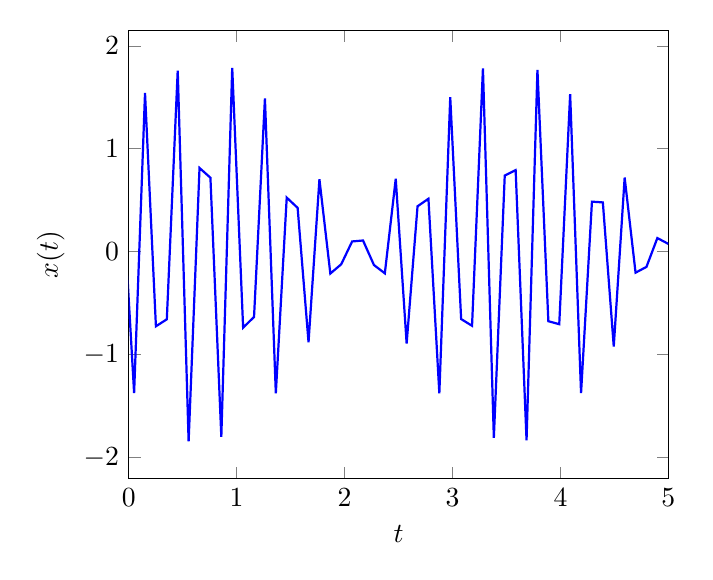
\begin{tikzpicture}
            \begin{axis}[xlabel={$t$}, ylabel={$x(t)$},xmin=0,xmax=5]
                \addplot[blue, thick, samples=100] {sin(deg(100*x)) + cos(deg(40*x))};
            \end{axis}
            \end{tikzpicture}
        }
        \caption{Resolución estándar}
    \end{subfigure}
    \hspace{0.05\textwidth} % espacio entre las figuras
    \begin{subfigure}[b]{0.45\textwidth}
        \centering
        \resizebox{\linewidth}{!}{%
            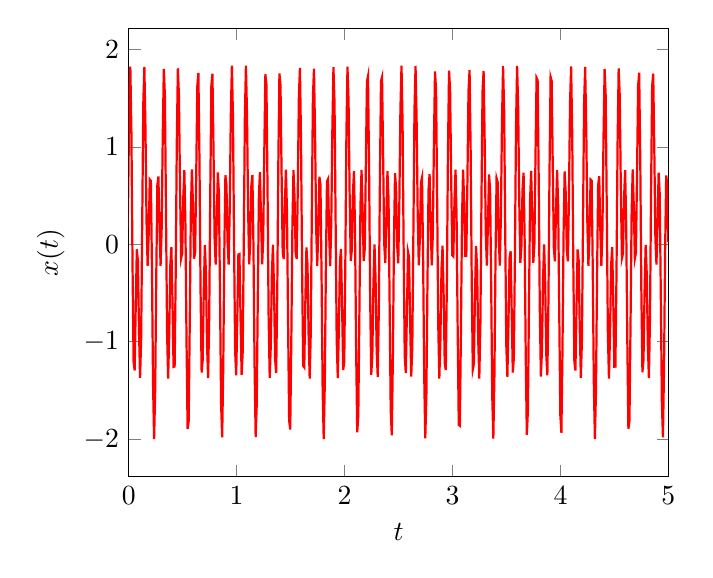
\begin{tikzpicture}
            \begin{axis}[xlabel={$t$}, ylabel={$x(t)$},xmin=0,xmax=5]
                \addplot[red, thick, samples=1000] {sin(deg(100*x)) + cos(deg(40*x))};
            \end{axis}
            \end{tikzpicture}
        }
        \caption{Resolución alta}
    \end{subfigure}

    \caption{Comparación de una señal con diferente cantidad de muestras}
    \label{fig:comparacion-muestras}
\end{figure}

